\setlength{\columnsep}{3pt}
\begin{flushleft}
	\bigskip
	\begin{figure}[h!]
		\centering
		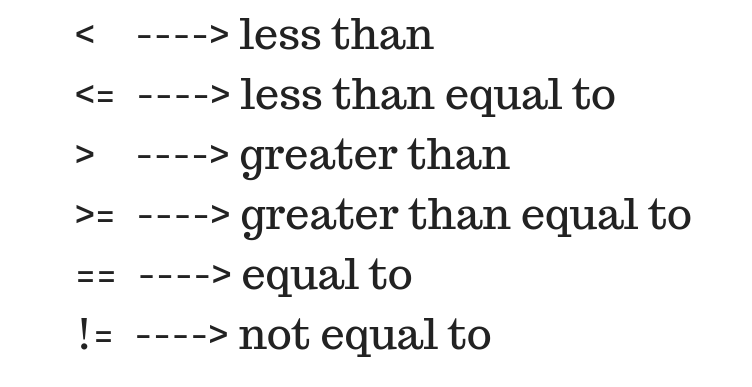
\includegraphics[scale=0.5]{content/chapter3/images/relational.png}
	\end{figure}

	\begin{tcolorbox}[breakable,notitle,boxrule=1pt,colback=yellow,colframe=yellow]
		\color{black}
		\fontdimen2\font=8pt
		\textbf{Note}: 
		\begin{itemize}
			\item \textbf{"<" , "<=" , ">" , ">="} are applicable on integers, strings \& boolean , but not on cross datatypes.	
			\item \textbf{"==" , "!="} are applicable on all datatypes, including cross datatypes.
			\item \textbf{"==" , "!="} never returns error.
		\end{itemize}
		\fontdimen2\font=4pt
	\end{tcolorbox}
	
	\newpage

	Sample code 1:
	\begin{tcolorbox}[breakable,notitle,boxrule=-0pt,colback=code,colframe=code]
			\color{white}
			\fontdimen2\font=8pt
			a=6 \newline
			b=2 \newline
			print(a>b, a<b) \newline
			a=6 \newline
			b=6 \newline
			print(a>=b, a<=b) \newline
			a="apple" \newline
			b="mango" \newline
			print(a>b, a<b)
			\fontdimen2\font=4pt
	\end{tcolorbox}
		
	Output:
	\begin{tcolorbox}[breakable,notitle,boxrule=-0pt,colback=output,colframe=output]
			\color{black}
			True False \newline
			True True \newline
			False True
			\fontdimen2\font=4pt
	\end{tcolorbox}
	\bigskip \bigskip
	Sample code 2:
		\begin{tcolorbox}[breakable,notitle,boxrule=-0pt,colback=code,colframe=code]
		\color{white}
		\fontdimen2\font=8pt
		a=6 \newline
		b="6" \newline
		print(a==b, a!=b) \newline
		a=6 \newline
		b=6 \newline
		print(a==b, a!=b)
		\fontdimen2\font=4pt
	\end{tcolorbox}
	
	Output:
	\begin{tcolorbox}[breakable,notitle,boxrule=-0pt,colback=output,colframe=output]
		\color{black}
		False True \newline
		True False
		\fontdimen2\font=4pt
	\end{tcolorbox}
\end{flushleft}

\newpage





